 
%{{{ Definimos parámetros iniciales
\documentclass{beamer}
\usepackage[english]{babel}
%\input{header2.tex}
\usepackage[utf8]{inputenc}
\usepackage{color}
\usetheme{Warsaw}
\usepackage{ragged2e} 
\usepackage{amssymb,amsmath}

\newcommand{\ket}[1]{\left| #1 \right>} % for Dirac bras
\newcommand{\bra}[1]{\left< #1 \right|} % for Dirac kets

\title[Quantum Computing]{An introduction}
\author{Oswaldo Gomez}
\institute{AI Engineering}
\date{\today}
\begin{document}
%}}}
%Start of slide
\begin{frame}{Quantum computing}
	\titlepage
\end{frame}

%Start of slide
\begin{frame}{Young's Double Slit Experiment}{Particles behave like waves}
	\center
	\begin{figure}
		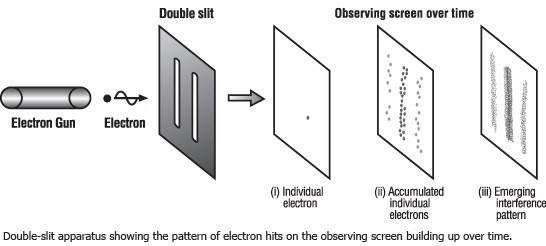
\includegraphics[keepaspectratio=true,width=.8\paperwidth]{.attachments/double-slit.jpeg}
		\caption{Image credit: ©2012 Perimeter Institute for Theoretical Physics, via https://www.perimeterinstitute.ca/research/research-areas/quantum-foundations/more-quantum-foundations.}
	\end{figure}
\end{frame}

%Start of slide
\begin{frame}{Quantum world if fascinating}{Particles behave like waves}
	\center
	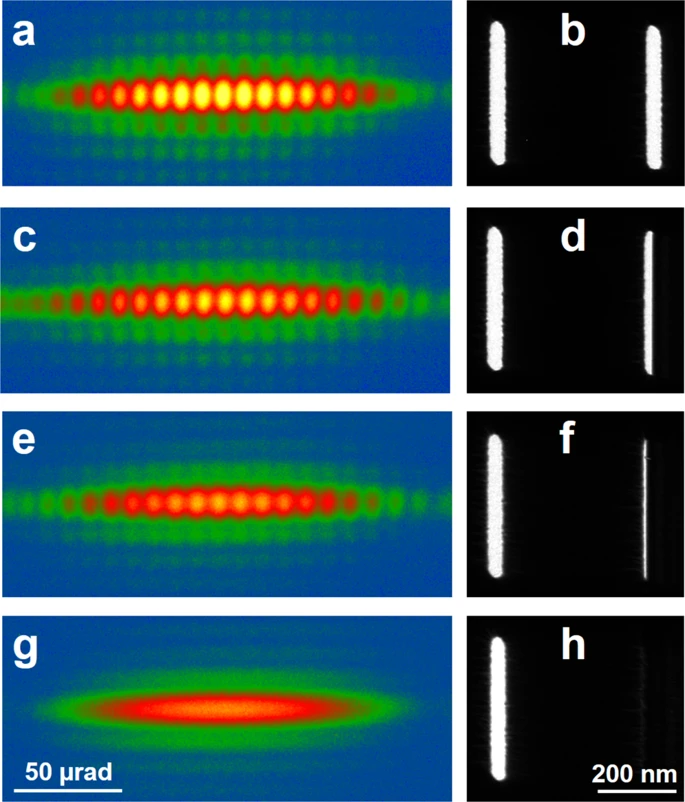
\includegraphics[keepaspectratio=true,width=.5\paperwidth]{.attachments/young.png}
\end{frame}

%Start of slide
\begin{frame}{Quantum world if fascinating}{Particles behave like waves}
	\justifying
	The state of a particle after passing through either one of the slits can be described as a \textit{wave} function (probability distribution) namely $\Psi = (\alpha_0 \psi_0 + \alpha_1 \psi_1)$ with $\{\alpha_0,\alpha_1\} \in \mathbb{C}$
	
	\center
	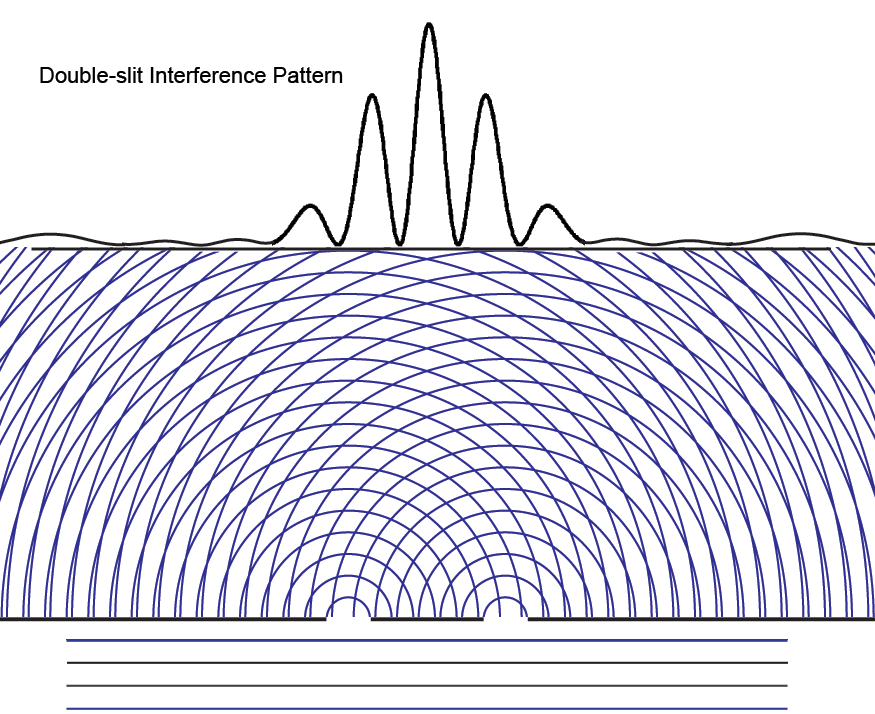
\includegraphics[keepaspectratio=true,width=.5\paperwidth]{.attachments/double-slit-distro.png}
\end{frame}


%Start of slide
\begin{frame}{Basic Unit of information: Bits}
	\justifying
	Traditional computation works with 0 and 1 as basic units of information. A physical realization of this is voltage from 0V to 5V
	\center
	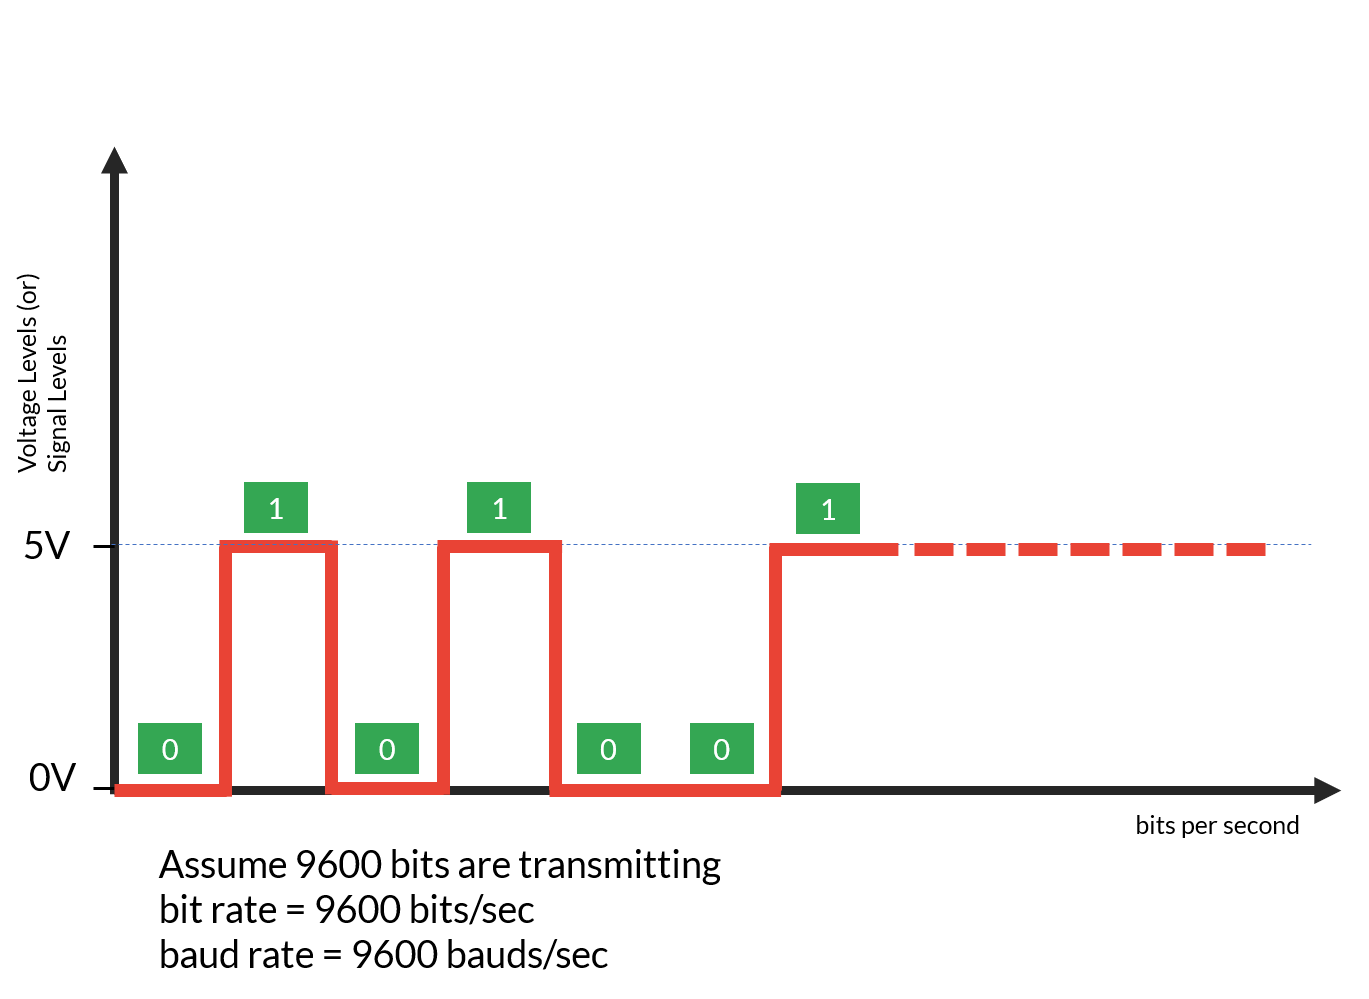
\includegraphics[keepaspectratio=true,width=.6\paperwidth]{.attachments/Bitrateequalbaudrate.png}
\end{frame}


%Start of slide
\begin{frame}{Basic Unit of information: Qubits}
	\justifying
	Quantum computation works with $\ket{0}$ and $\ket{1}$ as basic units of information. A physical realization of this would be a spin 1/2 particle.
		
	\center
	\includegraphics[keepaspectratio=true,width=.8\paperwidth]{.attachments/Qubit.png}
\end{frame}


%Start of slide
\begin{frame}{Computational basis states}
	\justifying
	Qubits can be in different states \textit{other} than $\ket{0}$ or $\ket{1}$. It is possible to form \textit{linear combinations} of states, called superpositions:
	$$\ket{\psi}= \alpha_0 \ket{0} + \alpha_1 \ket{1}$$
	The numbers $\alpha_0$ and $\alpha_1$ are complex numbers and ${|\alpha_0|}^2+|\alpha_1|^2=1$. 
	\newline
	\newline
	Where $\ket{0}$ and $\ket{1}$ are vectors $\begin{pmatrix} 1 \\ 0 \end{pmatrix}$ and $\begin{pmatrix} 0 \\1 \end{pmatrix}$ in ${\mathbb{C}}^2$.
	\newline
	\newline
	A superposition state is a linear combination $ \psi =\alpha_0 \begin{pmatrix} 1 \\ 0 \end{pmatrix} + \alpha_1 \begin{pmatrix} 0 \\ 1 \end{pmatrix}$
\end{frame}

%Start of slide
\begin{frame}{Quantum NOT gate}
	\justifying
	Classical computer circuits consists of wires and logic gates. E.g. the NOT gate which has a truth table $0 \rightarrow 1$ and $1 \rightarrow 0$.
	\newline
	\newline
	The analogous quantum operation would take
	
	$$\alpha_0 \ket{0} + \alpha_1 \ket{1} $$
	
	to 
	
	$$\alpha_0 \ket{1} + \alpha_1 \ket{0} $$
	\newline
	\newline
	Since a quantum state can be represented as a vector, we are looking for a matrix such that:
	$$\mathrm{X} \begin{bmatrix} \alpha_0 \\ \alpha_1 \end{bmatrix}=\begin{bmatrix} \alpha_1 \\ \alpha_0 \end{bmatrix}$$ 
\end{frame}



\begin{frame}{Quantum Gates}
	\justifying
	Quantum gates are represented by matrices applied on our vectors (qubits). Are all matrices valid Quantum Gates?...no.
	\newline
	\newline
	Recall that  ${|\alpha_0|}^2+|\alpha_1|^2=1$ for a quantum state 
	$$\alpha_0 \ket{0} + \alpha_1 \ket{1}$$.
	This must also hold for 
	$$\alpha_0^{'}  \ket{0} + \alpha_1^{'} \ket{1}$$
	after the gate has acted. It turns out that the appropriate condition on the matrix representing the gate is tha the matrix $U$ be unitary. That is (with $U^{\dagger}$ is the adjoint of $U$)
	$$U^{\dagger}U=I$$
	
\end{frame}	

\begin{frame}{Quantum Gates}
	\justifying 
	In classical computers we only have one non-trivial gate for one bit (NOT gate). In the case of Quantum computers we have many!
	\newline
	\newline
	For example the NOT gate:
	$$\mathrm{X} \equiv \begin{bmatrix} 0 & 1 \\ 
	1 & 0 \end{bmatrix}$$
	The $Haddamard$ gate
	$$\mathrm{H} \equiv \frac{1}{\sqrt{2}}\begin{bmatrix} 1 & 1 \\ 
	1 & -1 \end{bmatrix}$$
\end{frame}

\begin{frame}{Quantum Gates}
	\justifying 
	Some single qubit matrices are used quite frequently and are very useful.
	\center
	\begin{figure}
		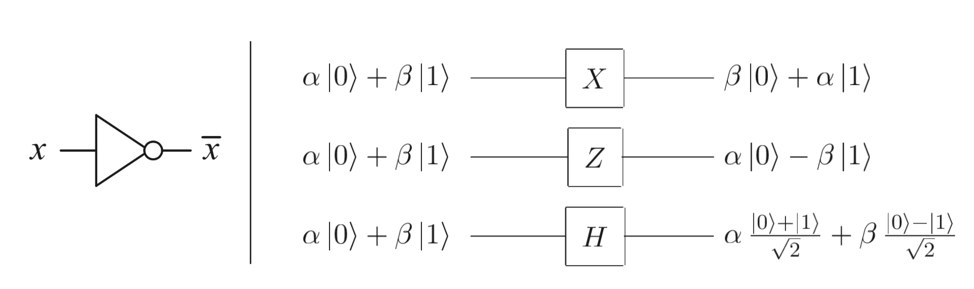
\includegraphics[keepaspectratio=true,width=.8\paperwidth]{.attachments/single_qubit.png}
		\caption{Single bit (left) and qubit (right) logic gates.}
	\end{figure}
\end{frame}

\begin{frame}{Two qubit representation}
	If $V$ and $W$ are vector spaces with bases $\{v_1...v_n\}$,$\{w_1...w_n\}$, the \textit{tensor product} $V \times W$ of $V$ and $W$ is a nm-dimensional vector space which is spanned by elements of the form $v\otimes w$.
	
	These elements behave bilinearly, meaning:
	
	$$
	\alpha(v \otimes w)=\alpha v \otimes w = v \otimes \alpha w 
	$$
	
	$$
	u \otimes v + w \otimes v = (u + w ) \otimes v
	$$
	
	$$
	u \otimes v + v \otimes w = u \otimes (v+w) 
	$$
	
	Using Dirack "ket" notation, we can write a two qubuit basis space as:
	
	$$
	\{\ket 0 \otimes \ket 0,\ket 0 \otimes \ket 1,\ket 1 \otimes \ket 0,\ket 1 \otimes \ket 1\}
	$$
\end{frame}



\begin{frame}{Problem to be solved by Deutsch's algorithm}
	\justifying 
	Given a black box $U_f$ implementing some unknown function $f : \{0, 1\}\rightarrow \{0, 1\}$, determine wheter $f$ is "constant" or "balanced". 
	\newline
	\newline
	Here "constant" means $f$ always outputs the same bit, i.e. $f(0)=f(1)$, and "balanced" means f outputs different bits on different inputs, i.e. $f(0) \neq f(1)$.
	\newline
	\newline
	There is an easy solution, simply evaluate $f$ on inputs 0 and 1, i.e. compute $f(0)$ and $f(1)$, and then check if $f(0)=f(1)$. This is the "classical" solution which requires two "queries" or calls to $U_f$. Can we solve it in just one query? 
	\newline
	\newline
	Classically, the answer turns out to be no. But quantumly this can be achieved in a single query
\end{frame}

\begin{frame}{A bit about black boxes}
	\justifying
	First we need to understand how to model a function in the quantum world. It turns out postulate 2 of quantum mechanics says, all quantum operations must be unitary and hence reversible.
	\newline
	\newline
	This is a bit non-trivial since in general given the output of a function $f(x)$, it is not always possible to invert $f$ to obtain $x$. We have to compute $f(x)$ in such a way as to guarantee that the computuation can be undone. This is achieved in the following setup:
	\begin{figure}
		\includegraphics[keepaspectratio=true,width=.6\paperwidth]{.attachments/oracle.png}
		\caption{$U_f$ is a unitary operator mapping $\ket x \ket y \rightarrow \ket x \ket {x \oplus y}$ for any $x,y \in \{\ket x, \ket y \}$} 
	\end{figure}
\end{frame}

\begin{frame}{A naive idea}
	\justifying
	Since we are leveraging Quantum Mechanics, what happens if we query $U_f$ with input state $\ket x$ replaced with  $\alpha \ket 0 + \beta \ket 1$ and output state $\ket y$ with $\ket 0$?
	\newline
	\newline
	Intuitively, we have set the input register to both inputs 0 and 1, so we expect $U_f$ to return a supersposition of both possible outputs, $f(0)$ and $f(1)$. Inded, by linearity of $U_f$, the output of the circuit will beamer
	\begin{align}
	\ket {\psi} &= U_f(\alpha \ket 0 + \beta \ket 1) \otimes \ket 0 = \alpha U_f \ket 0 \ket 0 + \beta U_f \ket 1 \ket 0 \nonumber \\
	&= \alpha \ket 0 \ket {f(0)} +  \beta \ket 1 \ket {f(1)} \nonumber
	\end{align}
	Great! We seem to have obtained both outputs of $f$ with just a single query! Unfortunately, upon measurement, we would only be able to obtain information about one of the two terms in superposition.
\end{frame}

\begin{frame}{Deutsch's algorithm}
	\justifying
	We failed obtaining $f(0)$ and $f(1)$ simultaneously. Luckily our goal is not that, but evaluating $f(0) \oplus f(1)$ will help us deterimine if our function is constant or balanced. The solution is Deutsch's algorithm
	\begin{figure}
		\includegraphics[keepaspectratio=true,width=.8\paperwidth]{.attachments/d_algorithm.png}
		\caption{Quantum circuit implementing Deutsch's algorithm}
	\end{figure}
\end{frame}

\begin{frame}{(Quantum) walk through}
	Not obvious at all why it works (generally true about all quantum algorithms). Let's first look at the start of the circuit ($\ket {\psi_0} $), then after applying the Haddamards ($\ket {\psi_1} $), then after applying $U_f$ ($\ket {\psi_2} $) and after applying the last Hadamard ($\ket {\psi_3} $)
	\newline
	\newline
	\begin{align}
		\ket {\psi_0} &= \ket{0} \ket{1},\nonumber \\
		\ket {\psi_1} &= \ket{+}\ket{-} = \frac{1}{2}(\ket{0}\ket{0}-\ket{0}\ket{1}+\ket{1}\ket{0}-\ket{1}\ket{1}) \nonumber
	\end{align}
	After applying the operator $U_f$, we have 
	$$
	\ket {\psi_2} = \frac{1}{2}(\ket{0}\ket{f(0)}-\ket{0}\ket{1+f(0)}+\ket{1}\ket{f(1)}-\ket{1}\ket{1+f(1)}) 
	$$
\end{frame}

\begin{frame}{Constant $f$}
	\justifying
	By definition, if $f$ is constant, then $f(0)=f(1)$ So we can simplify $\ket{\psi_2}$ as follows
	\begin{align} 
		\ket{\psi_2} &= \frac{1}{2} (\ket{0}\ket {f(0)}- \ket{0}\ket{1 \oplus f(0)} + \ket{1}\ket{f(0)} - \ket{1}\ket{1 \oplus f(0)}           ) \nonumber \\
		&= \nonumber \frac{1}{2} ((\ket {0}+ \ket{1}) \otimes \ket{f(0)} -  (\ket {0}+ \ket{1}) \otimes \ket{1 \oplus f(0)})\\
		&= \nonumber \frac{1}{2} (\ket {0}+ \ket{1}) \otimes (\ket{f(0)}-\ket{1 \oplus f(0)}) \\
		&= \nonumber \frac{1}{\sqrt{2}}\ket{+} \otimes (\ket{f(0)}-\ket{1 \oplus f(0)} )\\
	\end{align}
	Applying the last Haddamard on the top qubit we obtain:
	$$
	\ket{\psi_3}=\frac{1}{\sqrt{2}}\ket{0} \otimes (\ket{f(0)}-\ket{1 \oplus f(0)})
	$$
\end{frame}

\begin{frame}{Balanced $f$}
	\justifying
	By definition, if $f$ is constant, then $f(0) \neq f(1)$. Since f is a binary function, this means $f(0) \oplus 1 = f(1)$ and $f(1) \oplus 1 = f(0)$ we can then simplify:
	\begin{align} 
		\ket{\psi_2} &= \frac{1}{2} (\ket{0}\ket {f(0)}- \ket{0}\ket{f(1)} + \ket{1}\ket{f(1)} - \ket{1}\ket{f(0)}           ) \nonumber \\
		&= \nonumber \frac{1}{2} ((\ket {0}- \ket{1}) \otimes \ket{f(0)} -  (\ket {0}- \ket{1}) \otimes \ket{ f(1)})\\
		&= \nonumber \frac{1}{2} (\ket {0}- \ket{1}) \otimes (\ket{f(0)}-\ket{ f(1)}) \\
		&= \nonumber \frac{1}{\sqrt{2}}\ket{-} \otimes (\ket{f(0)}-\ket{ f(1)} )\\
	\end{align}
	Applying the last Haddamard on the top qubit we obtain:
	$$
	\ket{\psi_3}=\frac{1}{\sqrt{2}}\ket{1} \otimes (\ket{f(0)}-\ket{ f(1)})
	$$
\end{frame}

\begin{frame}{Final thoughts}
	\justifying
	Even though this quantum algorithm reduces "only" in half the amount of queries we have to make to our function. It turns out that there are other algorithms which provide an exponential advantage which use some of the ideas presented here.
	\newline
	\newline
	The fasinating world of quantum is finally begining to yield some of the advantages that I was not expecting to come to life during my lifetime.
	\newline
	\newline
	Incredibly we can now leverage real quantum computers and the future of Quantum Computing seems more realistic than 4 years ago (https://quantum-computing.ibm.com/)
\end{frame}

\begin{frame}{References}
	\begin{itemize}
		\item What is bit rate and baud rate with examples – bytesofgigabytes.com. (2019). Retrieved 20 January 2020, from http://www.bytesofgigabytes.com/embedded/bit-rate-and-baud-rate/
		      \newline
		\item {Nielsen, M., \& Chuang, I. (2010). Quantum Computation and Quantum Information: 10th Anniversary Edition. Cambridge: Cambridge University Press. doi:10.1017/CBO9780511976667}
		      \newline
		\item {Gulde, S., Riebe, M., Lancaster, G. et al. Implementation of the Deutsch–Jozsa algorithm on an ion-trap quantum computer. Nature 421, 48–50 (2003) doi:10.1038/nature01336}
\end{itemize}
\end{frame}



\begin{frame}{References}
	\begin{itemize}
\item Tavabi, A., Boothroyd, C., Yücelen, E., Frabboni, S., Gazzadi, G., Dunin-Borkowski, R., \& Pozzi, G. (2019). The Young-Feynman controlled double-slit electron interference experiment. Scientific Reports, 9(1). doi: 10.1038/s41598-019-43323-2
\item $Collapse of the Wave Function. (2020). Retrieved 21 January 2020, from http://www.informationphilosopher.com/solutions/experiments/wave-function_collapse/$
\item http://www.people.vcu.edu/~sgharibian/courses/CMSC491/notes/Lecture%206%20-%20Deutsch%27s%20algorithm.pdf
\end{itemize}
\end{frame}

\end {document}

